\subsection{Ringlicht}

Wird  ein  Objekt  von allen Seiten beleuchtet aber nicht von Oben, so  werden
Gravierungen sehr gut hervorgehoben (siehe Abbildung \ref{fig:muenzen}).

\begin{figure}[h!]
    \centering
    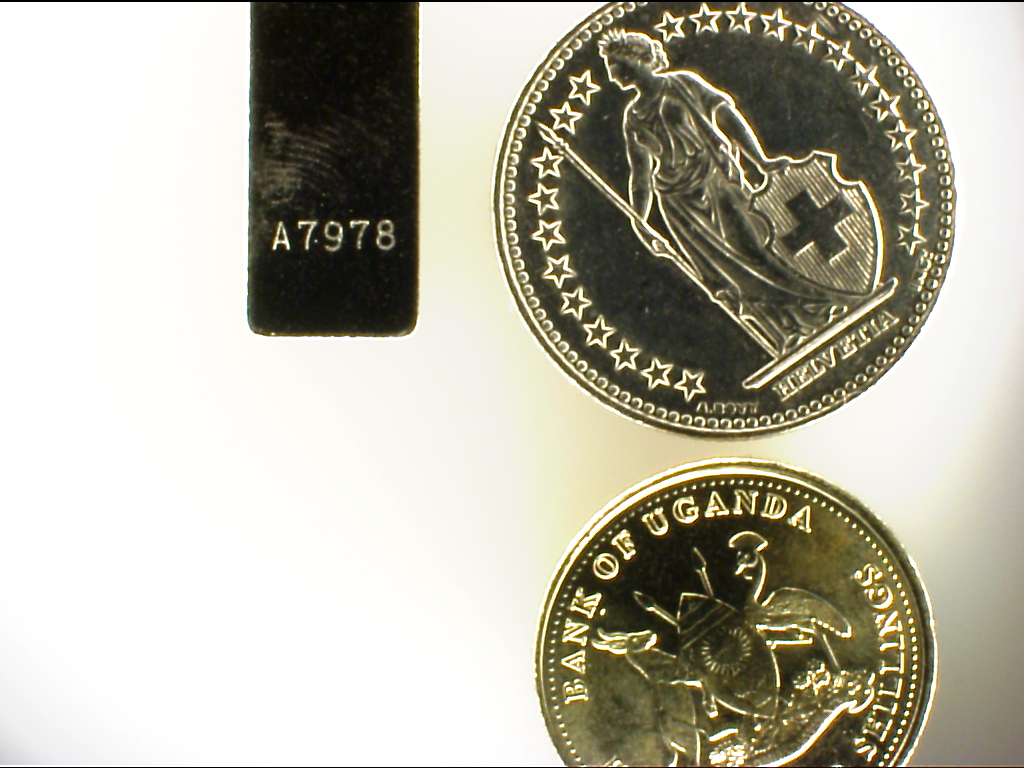
\includegraphics[width=.6\linewidth]{Posten_3_1_a_meme_1.png}
    \caption{Gravierungen sind sehr gut ersichtlich. Von Auge sieht man die Zahl ``A7978'' kaum.}
    \label{fig:muenzen}
\end{figure}


\subsection{Durchlichtbeleuchtung}

Mit Durchleuchtung  von Objekten lassen sich Materialien, die von Aussen nicht
sichtbar sind, hervorheben, weil  sie  das  durchleuchtende  Licht  blockieren
(siehe Abbildungen \ref{fig:note1} und \ref{fig:note2}).

\begin{figure}[h!]
    \centering
    \begin{subfigure}[b]{.45\linewidth}
        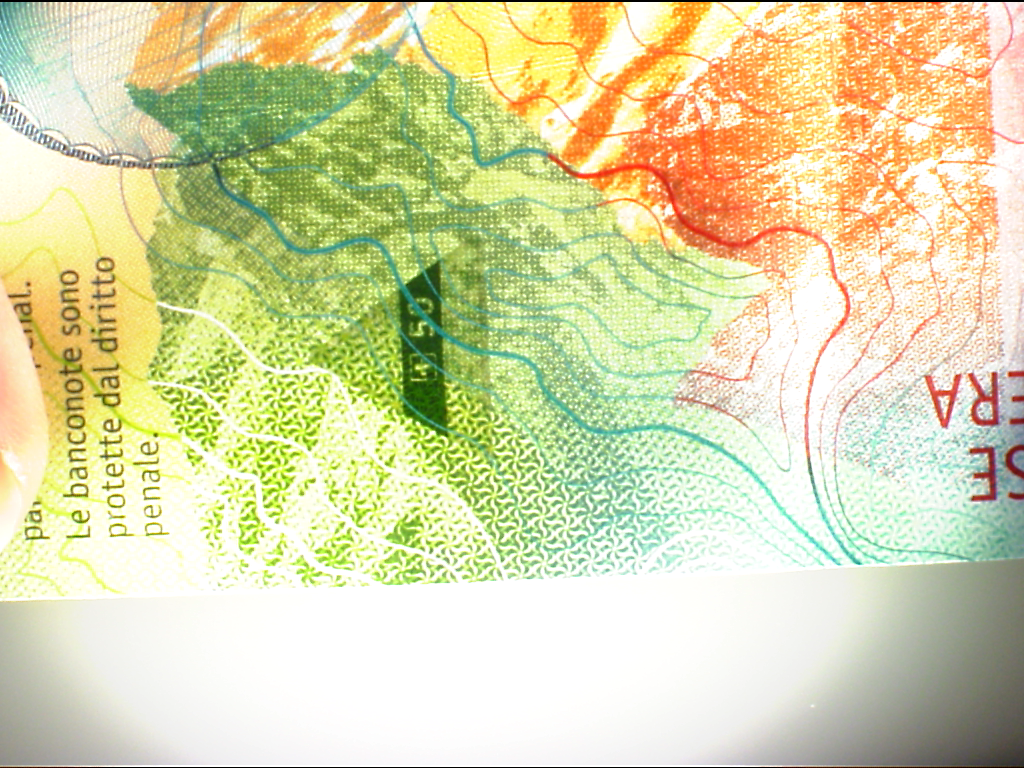
\includegraphics[width=\linewidth]{Posten_3_1_illuminati_invis}
        \caption{Das Band ist ohne Durchleuchtung nicht sichtbar.}
        \label{fig:note1}
    \end{subfigure}
    \begin{subfigure}[b]{.45\linewidth}
        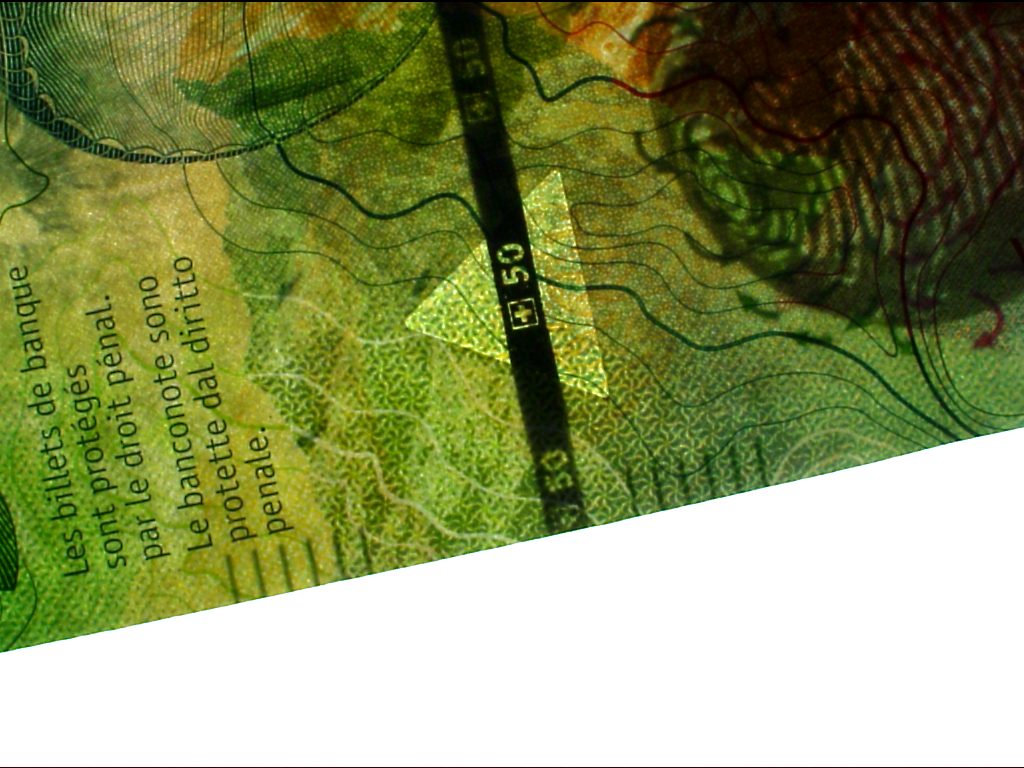
\includegraphics[width=\linewidth]{Posten_3_1_illuminati_visible}
        \caption{Mit Durchleuchtung wird das Band nun sichtbar.}
        \label{fig:note2}
    \end{subfigure}
\end{figure}


\newpage
\subsection{Polfilter}

Die  Lichtquelle   erzeugt   polarisiertes  Licht,  welches  von  der  M\"unze
reflektiert wird. Unter  Verwendung  eines  Polfilters kann das reflektierende
polarisierte Licht herausgefiltert werden.

\begin{figure}[h!]
    \centering
    \begin{subfigure}[b]{.45\linewidth}
        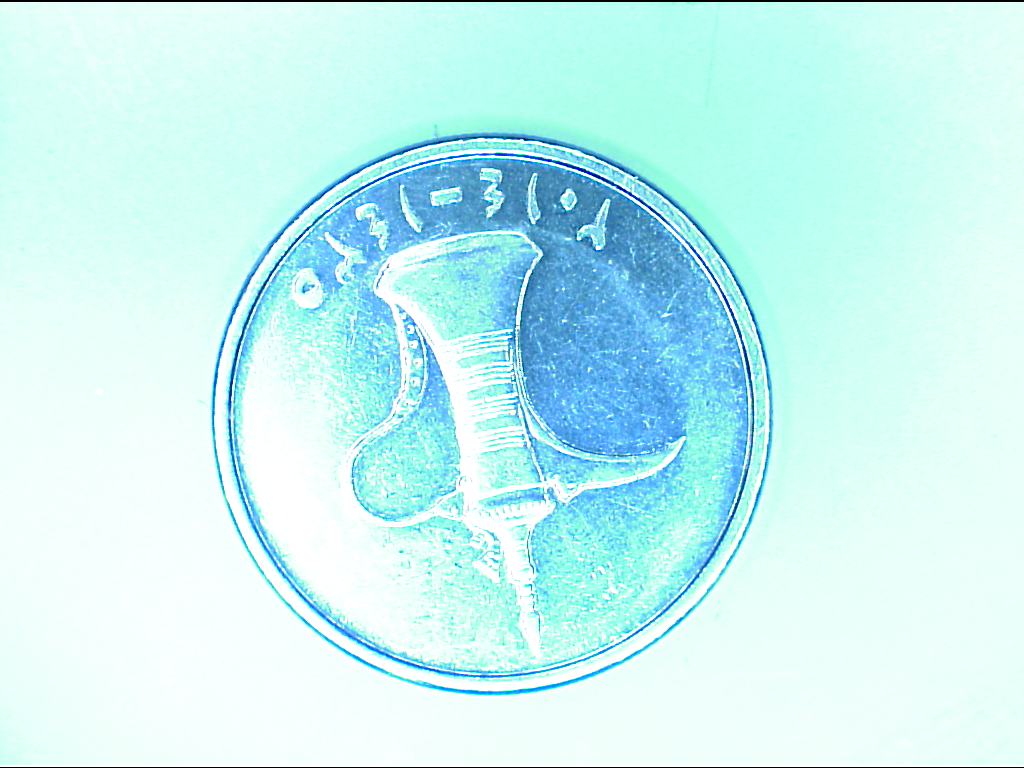
\includegraphics[width=\linewidth]{Posten_3_2_d_Reflektion_Stellung1}
        \caption{Ohne Polfilter}
    \end{subfigure}
    \begin{subfigure}[b]{.45\linewidth}
        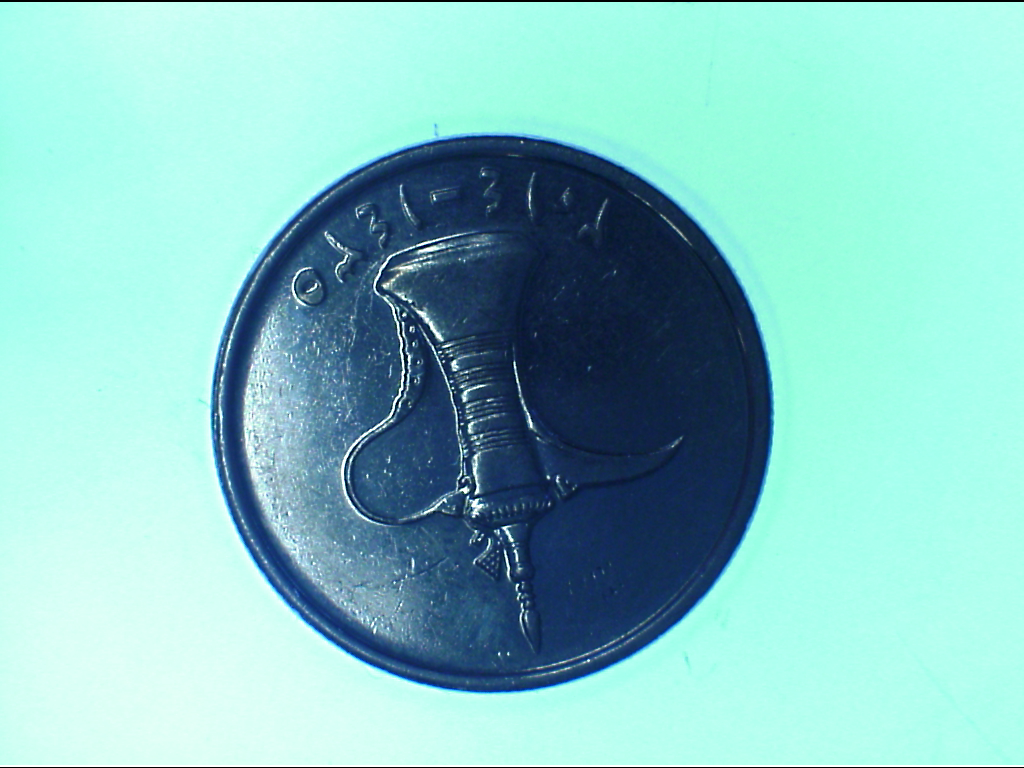
\includegraphics[width=\linewidth]{Posten_3_2_d_Reflektion_Stellung2}
        \caption{Mit Polfilter}
    \end{subfigure}
\end{figure}


\subsection{Dombeleuchtung}

Die  Dombeleuchtung  hebt  wie beim Ringlicht die Gravur der  M\"unze  hervor.
Dabei ist zu beachten dass kein Streulicht in  die  Dom  eindringt, was in den
Abbildungen \ref{fig:dom1} und \ref{fig:dom2} zu sehen ist.

\begin{figure}[h!]
    \centering
    \begin{subfigure}[t]{.45\linewidth}
        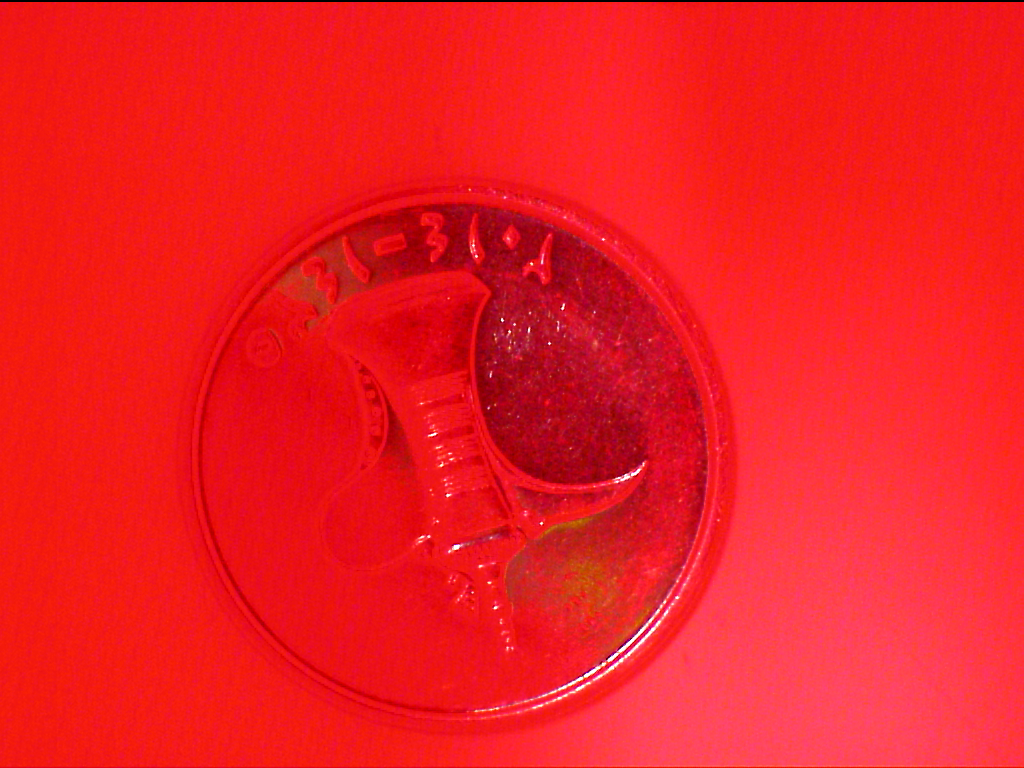
\includegraphics[width=\linewidth]{Posten_3_2_Reflektion_dom_rot}
        \caption{Mit einfallendem Streulicht}
        \label{fig:dom1}
    \end{subfigure}
    \begin{subfigure}[t]{.45\linewidth}
        
\includegraphics[width=\linewidth]{Posten_3_2_c_Reflektion_dom_rot}
        \caption{Abgedeckter Dom (kein einfallendes Streulicht, ausschliesslich Rot)}
        \label{fig:dom2}
    \end{subfigure}
\end{figure}


